%%%%%%%%%%%%%%%%%%%%%%%%%%%%%%%%%%%%%%%%%%%%%%%%
% E.Pinault-Bigeard - e.pinault-bigeard@upsti.fr
% http://s2i.pinault-bigeard.com
% CC BY-NC-SA 2.0 FR - http://creativecommons.org/licenses/by-nc-sa/2.0/fr/
%%%%%%%%%%%%%%%%%%%%%%%%%%%%%%%%%%%%%%%%%%%%%%%%
\documentclass[11pt]{article}
%%%%%%%%%%%%%%%%%%%%%%%%%%%%%%%%%%%%%%%%%%%%%%%%
% Package UPSTI_Document
%%%%%%%%%%%%%%%%%%%%%%%%%%%%%%%%%%%%%%%%%%%%%%%%
%%%%%%%%%%%%%%%%%%%%%%%%%%%%%%%%%%%%%%%%%%%%%%%%
% Package UPSTI_Document
%%%%%%%%%%%%%%%%%%%%%%%%%%%%%%%%%%%%%%%%%%%%%%%%
\usepackage{subcaption}
\usepackage[usenames, svgnames, dvipsnames]{xcolor}
\usepackage{UPSTI_Document}
\usepackage{pgfplots}
\definecolor{darkspringgreen}{rgb}{0.09, 0.45, 0.27}

\newcommandx*{\dessinRepereFigGeo}[5][1=\vx{},2=\vy{},3=\vz{},4=,5=0]
	{
		\draw [->,very thick] (0,0) -- (1,0) ;
		\draw [->,very thick] (0,0) -- (0,1) ;
    \fill[white] (0,0) circle (0.13);
    \draw [->,very thick] (0,0) circle (0.13);
    \ifnumequal{#5}{0} {% z vers nous
      \fill[black] (0,0) circle (0.03);
      \draw [->,thick] (0,0) circle (0.04);
    }{% z vers la feuille
  		\begin{scope} [rotate=45]
  			\draw [-,thick] (0,-0.12) -- (0,0.12) ;
  			\draw [-,thick] (-0.12,0) -- (0.12,0) ;
  		\end{scope}
    }
		\draw [anchor=north west] (1.1,0) node {${#1}$};
		\draw [anchor=south west] (0,1.1) node {${#2}$};
		\draw [anchor=north east] (-0.1,0) node {${#3}$};
		\draw [anchor=north west] (-0.1,-0.1) node {${#4}$};
	}

	\usepackage{array}
	\newcolumntype{L}[1]{>{\raggedright\let\newline\\\arraybackslash\hspace{0pt}}m{#1}}
	\newcolumntype{C}[1]{>{\centering\let\newline\\\arraybackslash\hspace{0pt}}m{#1}}
	\newcolumntype{R}[1]{>{\raggedleft\let\newline\\\arraybackslash\hspace{0pt}}m{#1}}

	\usepackage{pifont}% http://ctan.org/pkg/pifont
\newcommand{\cmark}{\color{green}\ding{51}}%
\newcommand{\xmark}{\color{red}\ding{55}}%
\newcommand{\fmark}{\ding{229}}%
\newcommand{\itemc}{\item[\cmark]}%
\newcommand{\itemx}{\item[\xmark]}%
\newcommand{\itemf}{\item[\fmark]}%


%---------------------------------%
% Paramètres du package
%---------------------------------%

% Version du document (pour la compilation)
% 1: Document prof
% 2: Document élève
% 3: Document à publier
\newcommand{\UPSTIidVersionDocument}{2}


% Classe
% 1: PTSI				6: PSI*			11: TSI2		16: Spé
% 2: PT	(par défaut)	7: MPSI			12: ATS
% 3: PT*				8: MP			13: PC
% 4: PCSI				9: MP*			14: PC*
% 5: PSI				10: TSI1		15: Sup
%\newcommand{\UPSTIidClasse}{2}

% Affichage personnalisé de la classe
\newcommand{\UPSTIclasse}{LP SARII}
\newcommand{\UPSTIvariante}{7}

% Matière
% 1: S2I (par défaut)    2: IPT     3: TIPE
% 6: Vie au lycée
\newcommand{\UPSTIidMatiere}{0}
\newcommand{\UPSTIintituleMatiere}{Automatique}
\newcommand{\UPSTIsigleMatiere}{Autom}
% Type de document
% 0: Custom*				7: Fiche Métho de			14: Document Réponses
% 1: Cours (par défaut)		8: Fiche Synthèse    		15: Programme de colle
% 2: TD     				9: Formulaire
% 3: TP						10: Memo
% 4: Colle					11: Dossier Technique
% 5: DS						12: Dossier Ressource
% 6: DM						13: Concours Blanc
% * Si on met la valeur 0, il faut décommenter la ligne suivante:
%\newcommand{\UPSTItypeDocument}{Custom}
\newcommand{\UPSTIidTypeDocument}{1}

% Titre dans l'en-tête

% Affichage personnalisé de la classe
\newcommand{\UPSTIclasse}{DUT}

% Variante utilisée
\newcommand{\UPSTIvariante}{7}

% Titre dans l'en-tête

\newcommand{\UPSTItitreEnTete}{Automatismes industriels}
%\newcommand{\UPSTItitreEnTetePages}{}
\newcommand{\UPSTIsousTitreEnTete}{Programmation des automates}


% Titre
%\newcommand{\UPSTItitrePreambule}{Automatisme industriel}
\newcommand{\UPSTItitre}{Sructure d'un automate industriel}

% Durée de l'activité (pour DS, DM et TP)
\newcommand{\UPSTIduree}{2h}

% Note de bas de première page
%\newcommand{\UPSTInoteBasDePremierePage}{Geoffrey Vaquette}
% Numéro (ajoute " n°1" après DS ou DM)
\newcommand{\UPSTInumero}{1}

% Numéro chapitre
%\newcommand{\UPSTInumeroChapitre}{1}

% En-tête customisé
%\newcommand{\UPSTIenTetePrincipalCustom}{UPSTIenTetePrincipalCustom}

% Message sous le titre
\newcommand{\UPSTImessage}{Message sous le titre}


% Référence au programme
%\newcommand{\UPSTIprogramme}{\EPBComp \EPBCompP{B1-02}, \EPBCompP{B2-49}, \EPBCompS{B2-50}, \EPBCompS{B2-51}, \EPBCompP{C1-07}, \EPBCompP{C1-08}}

% Si l'auteur n'est pas l'auteur par défaut
%\renewcommand{\UPSTIauteur}{WWOOOOOOWW}

% Si le document est réalisé au nom de l'équipe
%\newcommand{\UPSTIdocumentCollegial}{1}

% Source
\newcommand{\UPSTIsource}{A. Juton, J. Deprez, J. Maillefert, G. Vaquette}

% Version du document
\newcommand{\UPSTInumeroVersion}{1.0}

%-----------------------------------------------
\UPSTIcompileVars		% "Compile" les variables
%%%%%%%%%%%%%%%%%%%%%%%%%%%%%%%%%%%%%%%%%%%%%%%%


%%%%%%%%%%%%%%%%%%%%%%%%%%%%%%%%%%%%%%%%%%%%%%%%
% Début du document
%%%%%%%%%%%%%%%%%%%%%%%%%%%%%%%%%%%%%%%%%%%%%%%%
\begin{document}
\UPSTIbuildPage

%\UPSTIobjectif{Durant cette activité, nous allons analyser une trame pour l'envoi d'informations sur une étiquette.}

\section{Introduction}
Les automates industriels programmables sont au coeur des systèmes automatisés de production ou de gestion technique du bâtiment.
A partir d'\textbf{d'informations} en provenance des \textbf{capteurs}, ils agissent sur un \textbf{produit} à l'aide d'\textbf{actionneurs}.

Les automates présentent les avantages et inconvénients suivants

\begin{minipage}[t]{.49\linewidth}
	\begin{itemize}
		\itemc Faible coût de développement
		\itemc Déploiement et modifications rapides
		\itemc Mécaniquement et électriquement robuste
	\end{itemize}
\end{minipage}\hfill
\begin{minipage}[t]{.49\linewidth}
	\begin{itemize}
		\itemx Equipement coûteux
		\itemx Encombrant
	\end{itemize}
\end{minipage}

La facilité et la rapidité de développement ainsi que sa robustesse et l'électronique optimisée par le fabricant rendent l'automate plus utilisé que le micro-controleur dans l'industrie de production et de gestion technique du bâtiment.

\section{Structures des systèmes automatisés}
\UPSTIaRetenir{%
	L'automate industriel constitue la \textbf{partie commande} d'un système industriel. Elle communique avec la \textit{partie opérative} en envoyant des \textit{commandes} aux \textbf{\color{green} pré-actionneurs} et reçoit des \textbf{\color{red} informations} de la part des capteurs.%
}

\UPSTIaRetenir{%
Les \textbf{entrées} de l'automate sont reliées aux \textbf{capteurs} du système.\\
Les \textbf{sorties} de l'automate sont reliées aux \textbf{pré-actionneurs} du système.}

La Figure~\ref{fig:structureAPI} illustre la communication entre l'automate et la partie opérative d'un système. Il aparaît également l'\textbf{I}nterface \textbf{H}omme \textbf{M}achine (\textbf{IHM}) permettant de communiquer avec les utilisateurs ainsi qu'un réseau informatique pour communiquer avec des ordinateurs, d'autres automates ou même tout appareil sur internet.

\begin{figure}[ht]
	\centering
	\input{tikz/structure.tikz}
	\caption{Sructure d'un système industriel}
	\label{fig:structureAPI}
\end{figure}

\subsection{Les actionneurs}
Un actionneur est un composant réalisant une conversion d'énergie afin d'agir sur le système. C'est lui qui réalise l'\textbf{action} du système, d'où son nom actionneur.

\UPSTIexemple{%
\begin{minipage}[b]{.49\textwidth}
\centering
	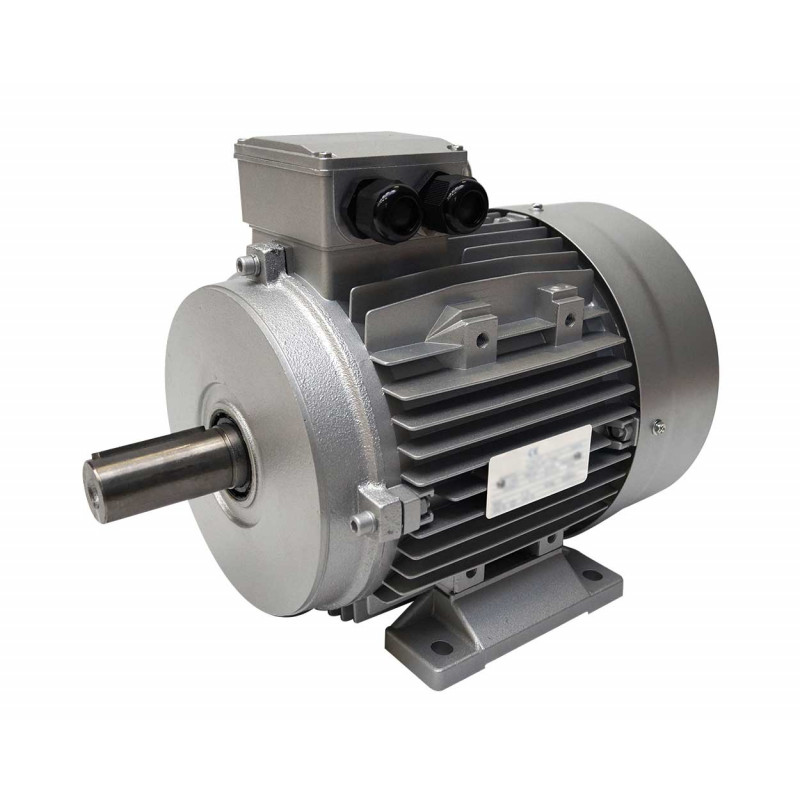
\includegraphics[width=.3\textwidth,height=.4\textheight,keepaspectratio]{images/moteur_electrique_triphase}

	Le moteur à courant continu converti l'énergie électrique en énergie mécanique.
\end{minipage}\hfill
\begin{minipage}[b]{.49\textwidth}
\centering
	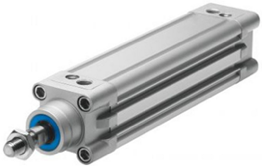
\includegraphics[width=.3\textwidth,height=.4\textheight,keepaspectratio]{images/verin_pneu}

	Un vérin pneumatique converti une énergie pneumatique en énergie mécanique.
\end{minipage}
 %
}

\subsection{Les pré-actionneurs}
Les \textbf{pré-actionneurs} remplissent la fonction \textit{distribuer} de la chaîne d'énergie. Ce sont eux qui  adaptent l'énergie puis la distubuent aux différents actionneurs. Ce sont eux qui \textbf{sont commandés par l'automate en vue de faire fonctionner les actionneurs}.

\UPSTIaRetenir{Un automate programmable \textbf{commande les pré-actionneurs} en vue de faire fonctionner les \textit{actionneurs}.}

\UPSTIexemple{%
\begin{minipage}[b]{.49\textwidth}
\centering
	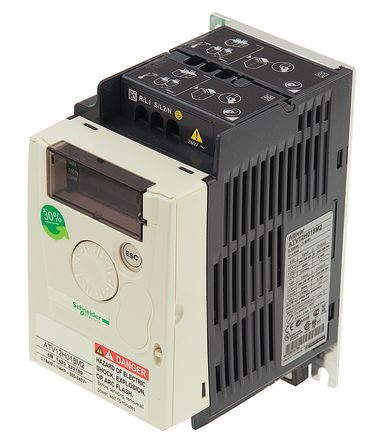
\includegraphics[width=.3\textwidth,height=.4\textheight,keepaspectratio]{images/varia_vitesse_mot_elec}

	Un variateur de vitesse pour moteur électrique adapte la tension d'alimentation du moteur pour en régler la vitesse.
\end{minipage}\hfill
\begin{minipage}[b]{.49\textwidth}
\centering
	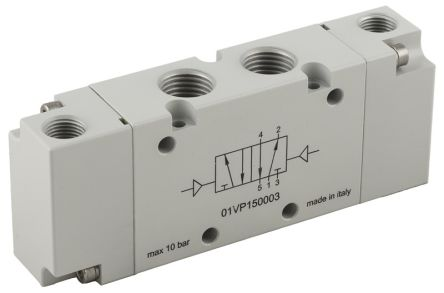
\includegraphics[width=.3\textwidth,height=.4\textheight,keepaspectratio]{images/distri_electroPneu}

	Un distributeur électro-pneumatique contrôle l'arrivée d'air comprimé dans les organes pneumatique (vérin par exemple).
\end{minipage}
 %
}

\subsection{Les capteurs}
Les capteurs sont des composants permettant d'acquérir une information en provenance du monde extérieur. Dans le cas d'un automate industriel, il permet de connaître l'état du système.

\UPSTIaRetenir{Un automate industriel acquiert des informations sur l'état d'un système à l'aide de \textbf{capteurs}}

\UPSTIexemple{%
\begin{minipage}[b]{.49\textwidth}
\centering
	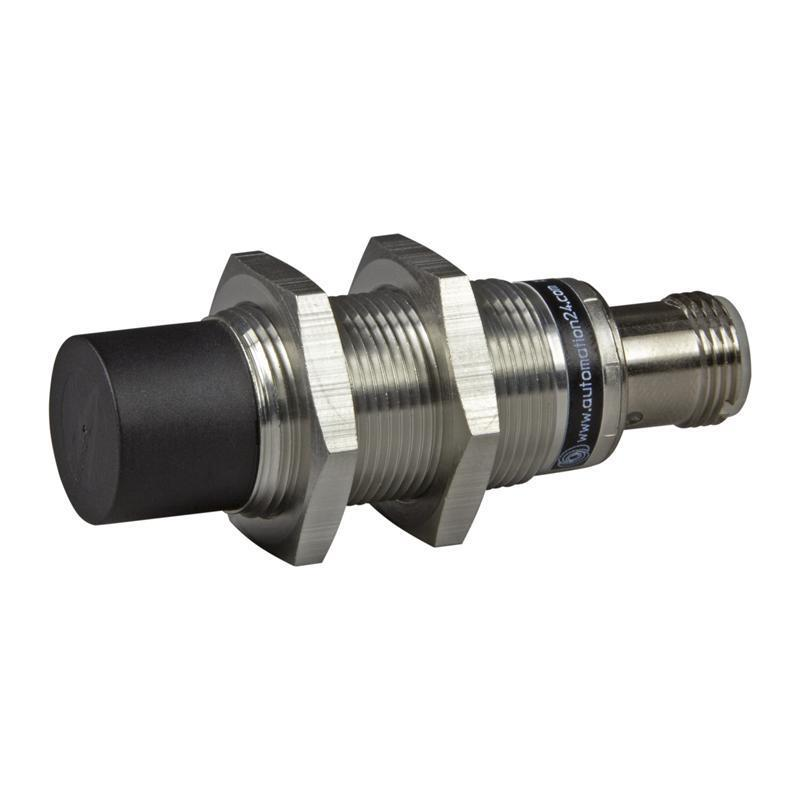
\includegraphics[width=.3\textwidth,height=.4\textheight,keepaspectratio]{images/capt_inductif}

	Un \textbf{capteur inductif} détecte la présence d'objets métalliques
\end{minipage}\hfill
\begin{minipage}[b]{.49\textwidth}
\centering
	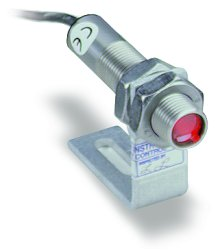
\includegraphics[width=.3\textwidth,height=.4\textheight,keepaspectratio]{images/capt_optique}

	Un capteur optique détecte la présence d'un objet à l'aide d'un faisceau optique.
\end{minipage}
\begin{minipage}[b]{.49\textwidth}
\centering
	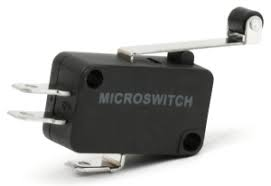
\includegraphics[width=.3\textwidth,height=.4\textheight,keepaspectratio]{images/detecteur_contact}

	Un capteur de contact détecte la présence d'un objet par contact.
\end{minipage}\hfill
\begin{minipage}[b]{.49\textwidth}
\centering
	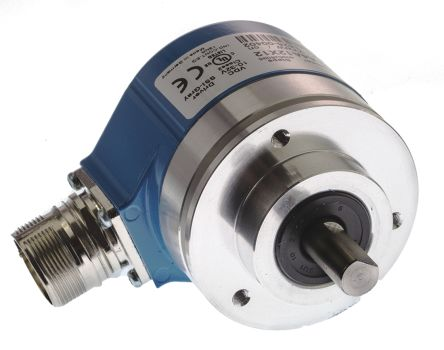
\includegraphics[width=.3\textwidth,height=.4\textheight,keepaspectratio]{images/codeur_optique}

	Un codeur optique renvoie des informations permettant de connaitre la position et la vitesse d'un moteur.
\end{minipage}
%
}

\subsection{Strucure locale et déportée}
Comme nous l'avons vu dans la section précédente, les automates industriels sont reliés aux capteurs et pré-actionneurs du système.

Sur les systèmes de petite taille et si l'installation le permet, les entrées et sorties de l'automate sont reliées directement à l'automate, on parle de \textbf{structure locale}. Pour des installations plus grande ou lorsque la configuration l'impose, les entrées et sorties sont reliées à des modules déportés (éloignés de l'automate), on parle de \textbf{structure déportée}. Ces deux configurations sont illustrée sur la Figure~\ref{fig:local_deporte}

\begin{figure}[h]
	\begin{subfigure}[b]{.49\textwidth}
		\centering
		\input{tikz/local_API.tikz}
		\caption{Strucure locale}
	\end{subfigure}
	\begin{subfigure}[b]{.49\textwidth}
	\centering
	\input{tikz/depoted_API.tikz}
	\caption{Strucure déportée}
	\end{subfigure}
	\caption{Strucure locale et déportée}
	\label{fig:local_deporte}
\end{figure}

Les bus de terrain reliant les modules peuvent être de différentes natures selon la configuration (CAN, Profibus, LON, BACNET, Ethernet, \dots).

\UPSTIaRetenir{%
\begin{description}
	\item [Sructure locale : ] Les entrées et sorties sont reliées à l'automate
	\item [Strucure déportée : ] Les entrées et sorties sont reliées à un module spécifique qui communique avec l'automate par un BUS de terrain.
\end{description}
}


\end{document}
